% Gage C. Linville | soils.land | gage@soils.land
\documentclass[12pt]{exam}
\newcommand{\semanticversion}{v1.0.0}                           % release version
\newcommand{\studentone}{Gage C. Linville}			% enter your name
%\newcommand{\studentemail}{}			                % enter your student email
\newcommand{\studentwebsite}{soils.land}                        % enter your website
\title{Soil Ecology Practice Exam}			        % change to the title of the project
\author{\studentone}				                % you don't have to change this
% Creation date
\newcommand{\creationdate}{April 1st, 2023}
% Revision date
\newcommand{\revisiondate}{May 10th, 2023}

%-------------------------------------------------------------------------------------
%  PACKAGES
%-------------------------------------------------------------------------------------
\usepackage{graphicx}
\usepackage{siunitx}
\usepackage{enumitem}

%-------------------------------------------------------------------------------------
%  GRAPHICS PATH
%-------------------------------------------------------------------------------------
\graphicspath{{figures/}}					% put your figures in a folder called figures

%---------------------------------------------------------------------------
% FUNCTIONS FOR IMPORTING FIGURES
%---------------------------------------------------------------------------
\newcommand{\placefigure}[1]{\centerline{\includegraphics[width=2 in]{#1}}}
\newcommand{\placefigureandscale}[2]{\centerline{\includegraphics[width=#2 in]{#1}}}

%-------------------------------------------------------------------------------------
% TITLE PAGE MACRO
%-------------------------------------------------------------------------------------
\makeatletter
\def\maketitle{%
  \null
  \thispagestyle{empty}
  \begin{center}\leavevmode
       \normalfont
       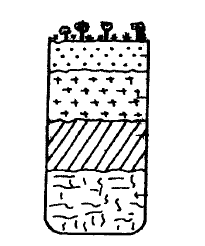
\includegraphics[width=0.20\columnwidth]{figures/Image_Edit.png}
%       \vskip 0.5cm
%       \textsc{\Large}\\[0.2 cm]
%       \vskip 0.3cm
	\rule{\linewidth}{0.2 mm} \\[0.4 cm]
	{ \huge \bfseries \@title}\\
	\rule{\linewidth}{0.2 mm} \\[0.4 cm]

	\begin{minipage}{0.5\textwidth}
		\begin{center} \large
			By: \studentone\\
            Created: \creationdate\\
            Revised: \revisiondate\\
            \semanticversion\\
%			\studentemail\\
%           \studentwebsite
			\end{center}
			\end{minipage}
   \end{center}
   \vfill
   \null
   \cleardoublepage
  }
\makeatother

%-------------------------------------------------------------------------------------
%	START OF DOCUMENT
%-------------------------------------------------------------------------------------

\begin{document}
%\large
\maketitle
%\frontmatter
\let\cleardoublepage\clearpage
%\mainmatter
\sloppy

%-------------------------------------------------------------------------------------
% CONTENTS
%-------------------------------------------------------------------------------------

\section*{15 Questions}
\begin{questions}
\question Which of following is classified as Mesofauna?

\begin{oneparchoices}
 \choice Protozoa
 \choice Mites %A
 \choice Algae
 \choice Root hairs
\end{oneparchoices}

\question Hermaphrodites are what?

\begin{choices}
 \choice Species of burrow dwellers without hair follicles
 \choice Egg eating organisms
 \choice Organisms without separate male and female genders %A
 \choice Polysaccharide dependant bacteria
\end{choices}

\question T/F Termite activity is on a scale comparable to that of earthworms.

\begin{oneparchoices}
 \choice True %A
 \choice False
\end{oneparchoices}

\question Nematodes of which genus can infest the roots of practically all plant species?

\begin{oneparchoices}
 \choice Pratylenchus
 \choice Trichinella
 \choice Capillaria
 \choice Heterodera %A
 \choice Trichuris
\end{oneparchoices}

\question What is the estimated number of protozoa species discovered so far?

\begin{oneparchoices}
 \choice 80,000
 \choice 25,000
 \choice 50,000 %A
 \choice 120,000
 \choice 70,000
\end{oneparchoices}

\question Briefly describe the rhizosphere.
\vspace{0.8in}

\question T/F Soil prokaryotes are only autotrophic.

\begin{oneparchoices}
 \choice True %A
 \choice False
\end{oneparchoices}

\question Cyanobacteria are unique because they contain which of the following?

\begin{oneparchoices}
 \choice Chlorophyll %A
 \choice Xylem vessels
 \choice Phloem tubes
 \choice Fungal mantle
\end{oneparchoices}
\newpage
\question Which of the following is phytotoxic?

\begin{oneparchoices}
 \choice K
 \choice Fe
 \choice Mn
 \choice Al %A
 \choice Ca
\end{oneparchoices}

\question List out the 17 essential plant nutrients.
\vspace{1in}
%A Carbon, Hydrogen, Oxygen, Calcium, Magnesium, Phosphorous, Potassium, Nitrogen, Sulfur, Iron, Zinc, Nickel, Copper, Boron, Chlorine, Molybdenum, Manganese.
\question Correctly identify \emph{two} eukaryotic organisms from the following:

\begin{oneparchoices}
 \choice Protozoa %A
 \choice Monera
 \choice Algae %A
 \choice Coccus
 \choice Stele
\end{oneparchoices}

\question Which is more physiologically diverse?

\begin{oneparchoices}
 \choice Eukaryotes
 \choice Prokaryotes %A
\end{oneparchoices}

\question Where are Methanogens known to be commonly found?

\begin{oneparchoices}
    \choice Contaminated soils
    \choice Acidic soils
    \choice Poorly drained soils %A
    \choice Salty conditions
\end{oneparchoices}

\question T/F It is thought that fungi and actinomycetes tend to prevail in desert soils due to their extensive filamentous growth.

\begin{oneparchoices}
 \choice True %A
 \choice False
\end{oneparchoices}

\question At what temperature are cells progressively killed?

\begin{oneparchoices}
 \choice \ang{25}C upward
 \choice \ang{35}C upward %A
 \choice \ang{9}C downward
 \choice \ang{2}C downward
\end{oneparchoices}
\end{questions}
\end{document}
